
\section{Non-Linear Single Tuned Mass Damper}
\begin{figure}[ht]
    \centering
    % \documentclass[border=1mm, class=article preview]{standalone}
\documentclass[border=3pt,tikz]{standalone}
\usepackage{tikz}
\usetikzlibrary{calc,patterns,decorations.pathmorphing,decorations.markings}

\begin{document}

% \begin{tikzpicture}[every node/.style={draw,outer sep=0pt,thick}, transform canvas={scale=1.0}]
\begin{tikzpicture}
% TikZ Styles
\tikzstyle{mass}=[draw,outer sep=0pt,thick]
\tikzstyle{spring}=[thick,decorate,decoration={zigzag,pre length=0.3cm,post length=0.3cm,segment length=6}]
\tikzstyle{damper}=[thick,decoration={markings,  
  mark connection node=dmp,
  mark=at position 0.5 with 
  {
    \node (dmp) [thick,inner sep=0pt,transform shape,rotate=-90,minimum width=15pt,minimum height=3pt,draw=none] {};
    \draw [thick] ($(dmp.north east)+(2pt,0)$) -- (dmp.south east) -- (dmp.south west) -- ($(dmp.north west)+(2pt,0)$);
    \draw [thick] ($(dmp.north)+(0,-5pt)$) -- ($(dmp.north)+(0,5pt)$);
  }
}, decorate]
\tikzstyle{ground}=[fill,pattern=north east lines,draw=none,minimum width=0.75cm,minimum height=0.3cm]
% Actual Drawing
\node (m2) [mass,minimum width=1.5cm,minimum height=1cm] {$m_2$};
\node (m1) at (m2.south) [mass,yshift=-1.5cm,anchor=north,minimum width=2cm,minimum height=1cm] {$m_1$};
\node (ground) at (m1.south) [ground,yshift=-1.5cm,anchor=north,minimum width=2cm] {};
\draw (ground.north west) -- (ground.north east);
\draw [spring] ([xshift=-0.5cm] ground.north) -- ([xshift=-0.5cm] $(m1.south east)!(ground.north)!(m1.south west)$) node[midway, left]{$k_1$};
\draw [damper] ([xshift=0.5cm] ground.north) -- ([xshift=0.5cm] $(m1.south east)!(ground.north)!(m1.south west)$) node[midway, right,xshift=2mm]{$c_1$};
\draw [spring] (m1.135) -- ($(m2.south east)!(m1.135)!(m2.south west)$) node[midway, left]{$k_{2c}$};
\draw [damper] (m1.45) -- ($(m2.south east)!(m1.45)!(m2.south west)$) node[midway, right,xshift=2mm]{$c_2$};
\draw [thick] (m1.east) -- +(0.5cm,0);
\draw [-latex,thick] ([xshift=0.5cm]m1.east) -- +(0,1cm) node[midway, right]{$f_1$};
\draw [thick] ([xshift=-0.25cm]m1.west) -- +(-0.5cm,0);
\draw [-latex,thick] ([xshift=-0.5cm]m1.west) -- +(0,1cm) node[midway, left]{$x_1$};
\draw [thick] ([xshift=-0.25cm]m2.west) -- +(-0.5cm,0);
\draw [-latex,thick] ([xshift=-0.5cm]m2.west) -- +(0,1cm) node[midway, left]{$x_2$};
\end{tikzpicture}

\end{document}
    \caption{\raggedright SDOF System with non-linear STMD}
    \label{fig:nlSTMD}
\end{figure}
\par Up to that section, we assumed that all the springs and dampers as linear devices. However, in reality none of them is truly linear. In addition to that, introducing non-linearity in a TMD may increase its performance. Due to those reasons, it is important to analyse non-linear TMDs. In that example, non-linearity is introduced with changing the linear spring with the non-linear one. For that spring, force and displacement function is $ F = x^3 \cdot k_{2c} $ instead of $ F = x \cdot k_2 $.
\subsection{Analysis}
EOM can be written as:\\
\begin{align*}
m_1 \ddot{x_1}+(c_1+c_2)\dot{x_1}-c_2\dot{x_2}+k_1x_1+k_{2c}(x_1-x_2)^3&=f_1\\
m_2 \ddot{x_2}-c_2\dot{x_1}+c_2\dot{x_2}-k_{2c}(x_1-x_2)^3&=0
\end{align*}
We can write the state-space representation as follows:
$$
\frac{d}{dt}\begin{Bmatrix}
 x_1\\
 x_2\\
 \dot{x_1}\\
 \dot{x_2}
\end{Bmatrix}=
\begin{Bmatrix}
 \dot{x_1}\\
 \dot{x_2}\\
 \ddot{x_1}\\
 \ddot{x_2}
\end{Bmatrix}=
\begin{Bmatrix}
 \dot{x_1}\\
 \dot{x_2}\\
 \frac{-(c_1+c_2)\dot{x_1}+c_2\dot{x_2}-k_1x_1-k_{2c}(x_1-x_2)^3+f_1sin(\omega t)}{m_1}\\
\frac{c_2\dot{x_1}-c_2\dot{x_2}+k_{2c}(x_1-x_2)^3}{m_2} 
\end{Bmatrix}
$$
For a given $ k_{2c} $, $ c_2 $ and $ \omega $ t is possible to solve that equation numerically using Runge Kutta Fehlberg method. Time domain solutions of the nonlinear system for the parameters $k_{2c} = 0.1 N/m^3$, $ c_2 = 0.05 N \cdot s / m $ and $ \omega = 0.8 rad/s $  and the optimum linear STMD can be seen at figure \ref{fig:nonlinearTimeDomain}. In that particular example, the response amplitude of the non-linear TMD is less than the response amplitude of the linear TMD.\\
\begin{figure}[ht]
    \centering
    \centerfloat
    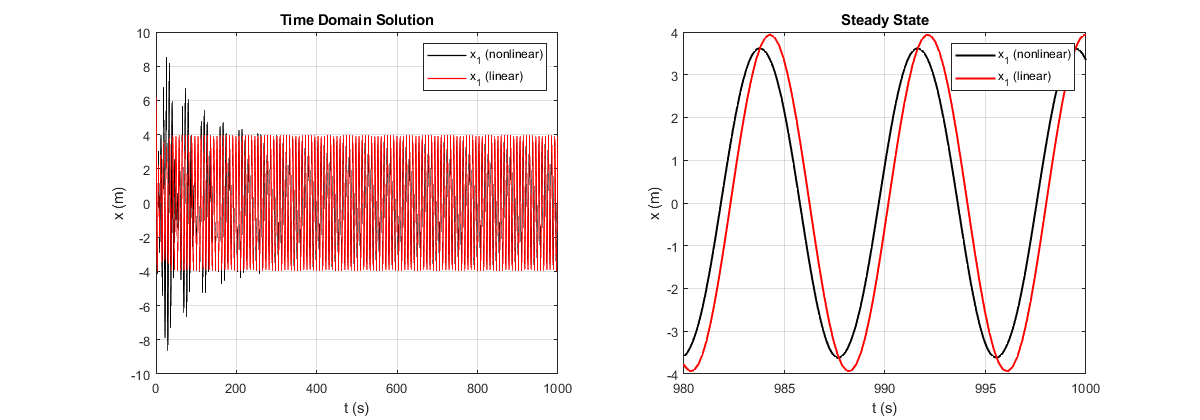
\includegraphics[scale=0.6]{MATLAB Figures/nonlinear time domain.png}
    \caption{Nonlinar STMD with optimum linear STMD}
    \label{fig:nonlinearTimeDomain}
\end{figure}
As seen on the figure \ref{fig:nonlinearTimeDomain}, both linear and non-linear systems are reaching the steady state after some time. We can find the frequency response of the non-linear system by finding the steady state amplitudes for a range of $ \omega $ values. The frequency response of the system can be seen at figure \ref{fig:freq_nlTMD}.
\begin{figure}[ht]
    \centering
    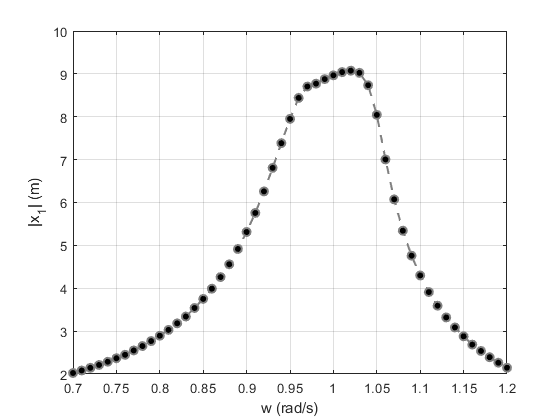
\includegraphics[scale=0.6]{MATLAB Figures/nonlinear stiffness.png}
    \caption{Frequency response of the nonlinear system}
    \label{fig:freq_nlTMD}
\end{figure}
\par In previous sections, we tried to optimize the peak value of the frequency response of the systems. Unfortunately, for the nonlinear system, we can't find the exact maximum since the frequency response function is unknown. However, what we can do is to take the maximum calculated value as the maximum in order to understand the behavior of the system for different TMD parameters. Finding the peak values for a grid of different TMD parameters ($k_{2c}$ and $c_2$) we can create a plot. It can be seen at figure \ref{fig:peak_nl}.\\
\begin{figure}
    \centering
    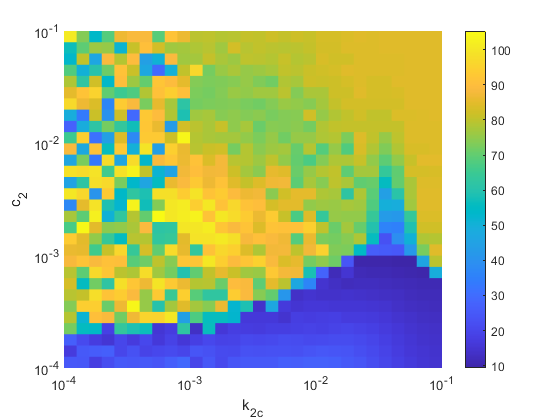
\includegraphics[scale=0.6]{MATLAB Figures/nonlinear peak.png}
    \caption{Peak values of the frequency response of the nonlinear TMD}
    \label{fig:peak_nl}
\end{figure}
\par The system shows a chaotic behavior especially at the top left part of the plot. At other areas it has more predictable behaviour. However, it is important to point out that this plot has some significant drawbacks due to the assumptions made at each step while creating it. This should be considered while interpreting the results.